\documentclass[12pt]{article}
\usepackage{geometry}                % See geometry.pdf to learn the layout options. There are lots.
\geometry{letterpaper}                   % ... or a4paper or a5paper or ... 
%\geometry{landscape}                % Activate for for rotated page geometry
\usepackage[parfill]{parskip}    % Activate to begin paragraphs with an empty line rather than an indent
\usepackage{daves,fancyhdr,natbib,graphicx,dcolumn,amsmath,lastpage,url}
\usepackage{amsmath,amssymb,epstopdf,longtable}
\usepackage[final]{pdfpages}
\DeclareGraphicsRule{.tif}{png}{.png}{`convert #1 `dirname #1`/`basename #1 .tif`.png}
\pagestyle{fancy}
\lhead{CE 3354 -- Engineering Hydrology}
\rhead{SUMMER 2025}
\lfoot{ES7}
\cfoot{}
\rfoot{Page \thepage\ of \pageref{LastPage}}
\renewcommand\headrulewidth{0pt}



\begin{document}
\begin{center}
{\textbf{{ CE 3354 Engineering Hydrology} \\ {Exercise Set 7}}}
\end{center}

\section*{\small{Exercises}}
\begin{enumerate}

\item Figure \ref{fig:OklahomaData} The following data represent gage height and annual peak discharge for some gaging station in Oklahoma.  The stage is in feet and the discharge is in cubic feet per second.  The data are sequential from 1923 through 1971.

\begin{figure}[h!] %  figure placement: here, top, bottom, or page
   \centering
   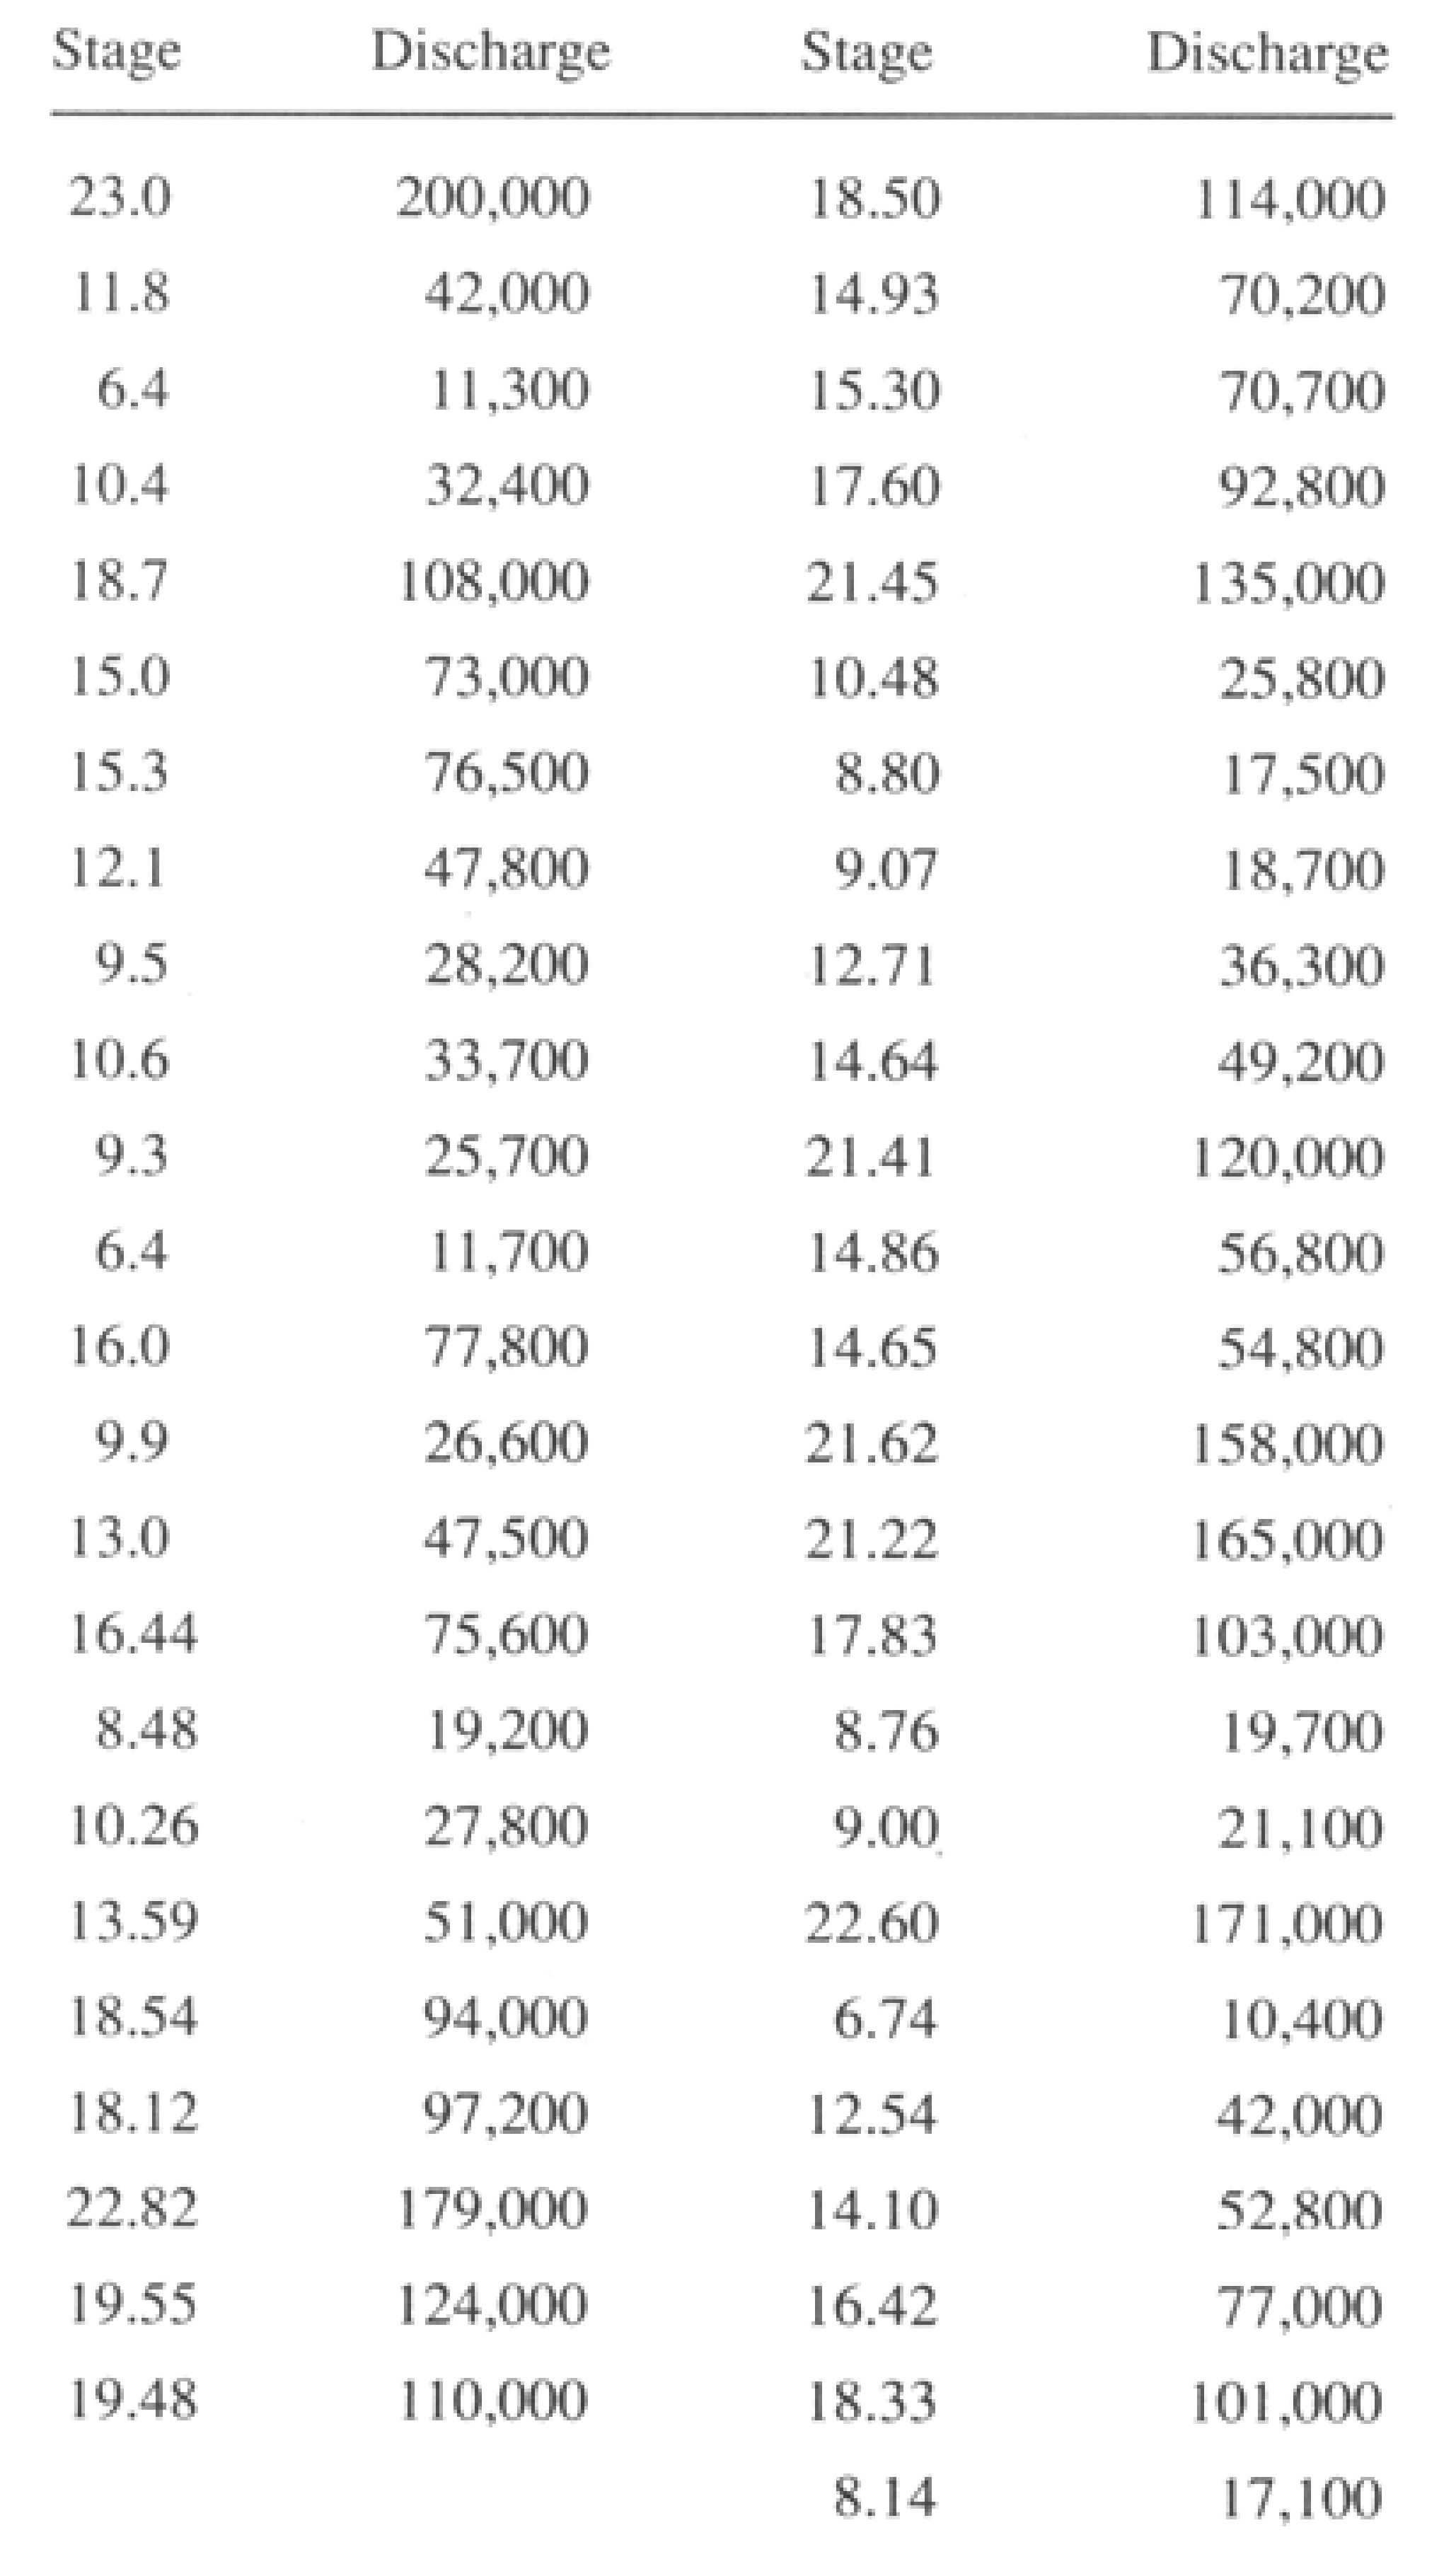
\includegraphics[height=7in]{OklahomaData.jpg} 
   \caption{Data from Oklahoma Gaging Station}
   \label{fig:OklahomaData}
\end{figure}

Use the data to:
\begin{enumerate}
\item Plot year versus stage ( x-axis is year).
\item Plot year versus discharge ( x-axis is year).
\item Plot the discharge versus stage.
\item Using the Weibull plotting position formula, determine the distribution parameters that fit the data for a log-normal distribution.
\item Using the Weibull plotting position formula, determine the distribution parameters that fit the data for a Gumbell distribution.
\item Using the Weibull plotting position formula, determine the distribution parameters that fit the data for a Gamma distribution.
\item Estimate the discharge associated with a 25-percent chance exceedence probability (i.e. the value that is equal to or exceeded with a 1 in 4 chance).
\item A resident claims that in the early 1900?s a flood corresponding to a stage of 30 feet occurred at the gage location.  Estimate the exceedence probability (return period) of the flow assicoated with this event.
\end{enumerate}
\clearpage

\item Use the Oklahoma data you just prepared and analyze using the Bulletin 17C procedure (using the PeakFQ software tool - use station skew option).   \\~\\ If starting from just the data in ES3 you will have to carefully build an input file -- the \textbf{Beargrass-B17C.txt}\footnote{This file is linked in the instructor notes; a formatted copy is included below.} file is the correct format. 

\item  Locate USGS Station 08144800 Brady Creek near Eden, TX. and analyze the historical peaks using the Bulletin 17C procedures (using the PeakFQ software tool use station skew option).  Determine the median discharge predicted for this station by PeakFQ.  Also determine the discharge per square mile of contributing drainage area.\footnote{Download the annual peaks from NWIS in the Watstore Format for use in peakFQ to avoid editing the file; a formatted copy (not current) is included below}

\end{enumerate}

\clearpage

\section*{\small{Oklahoma in PeakFQ format (minor editing may still be needed)}}
\begin{verbatim}
* WCF2.DATA  1/9/89 -- BULLETIN 17 EXAMPLES
*---+----1----+----2----+----3----+----4----+----5----+----6----+----7----+----8

Z                               USGS

*               LAT   LON                        AREA          ELEV
* STATIONID     DDMMSSDDDMMSS                    1234567123456712345678

H 12345678      3527470973329                    645.55        1202.01
N 12345678      OKLAHOMA WATERSHED
Y 12345678      20.0
2 12345678
3 12345678      19230101 200000
3 12345678      19240101 42000
3 12345678      19250101 11300
3 12345678      19260101 32400
3 12345678      19270101 108000
3 12345678      19280101 73000
3 12345678      19290101 76500
3 12345678      19300101 47800
3 12345678      19310101 28200
3 12345678      19320101 33700
3 12345678      19330101 25700
3 12345678      19340101 11700
3 12345678      19350101 77800
3 12345678      19360101 26600
3 12345678      19370101 47500
3 12345678      19380101 75600
3 12345678      19390101 19200
3 12345678      19400101 27800
3 12345678      19410101 51000
3 12345678      19420101 94000
3 12345678      19430101 97200
3 12345678      19440101 179000
3 12345678      19450101 124000
3 12345678      19460101 110000
3 12345678      19470101 114000
3 12345678      19480101 70200
3 12345678      19490101 70700
3 12345678      19500101 92800
3 12345678      19510101 135000
3 12345678      19520101 25800
3 12345678      19530101 17500
3 12345678      19540101 18700
3 12345678      19550101 36300
3 12345678      19560101 49200
3 12345678      19570101 120000
3 12345678      19580101 56800
3 12345678      19590101 54800
3 12345678      19600101 158000
3 12345678      19610101 165000
3 12345678      19620101 103000
3 12345678      19630101 19700
3 12345678      19640101 21100
3 12345678      19650101 171000
3 12345678      19660101 10400
3 12345678      19670101 42000
3 12345678      19680101 52800
3 12345678      19690101 77000
3 12345678      19700101 101000
3 12345678      19710101 17100         
*

\end{verbatim}

\clearpage
\section*{\small{Station 08144800 in PeakFQ format (minor editing may still be needed)}}
\begin{verbatim}
Z08144800                       USGS 
H08144800       3111030995027004848095SW12090110101    101     2000.99          
N08144800       Brady Ck nr Eden, TX
Y08144800       
308144800       19611009    2786               3.18                      
308144800       19630505   3.006               1.45                      
308144800       19631001   0.006                                         
308144800       19650518   57.06               2.24                      
308144800       19660428   51106               7.08                      
308144800       19670817   45606               6.72                      
308144800       19680310   11.06               1.78                      
308144800       19690911    9466               4.37                      
308144800       19700515   12.06               1.83                      
308144800       19710530   10206               4.04                      
308144800       19720615    3756               3.00                      
308144800       19730603    4106               3.07                      
308144800       19731012   33206               6.16                      
308144800       19750511    2446               3.07                      
308144800       19760711    4736               3.51                      
308144800       19770624   37206               6.45                      
308144800       19780528   38.06               1.84                      
308144800       19790809   10.06               1.51                      
308144800       19800909   13506               4.58                      
308144800       19810516   48.06               2.03                      
308144800       19820505    1776               2.71                      
308144800       19830606    1356               2.55                      
308144800       19840812    3336               3.14                      
308144800       19841231   60.06               2.08  
\end{verbatim}

\end{document}  